\documentclass[reqno, 12pt]{amsart}

\usepackage{amssymb, amsmath, amsthm, enumerate, mathtools, graphicx, enumitem, tikz, color, soul, bbm, verbatim, parskip, multicol}
\usepackage[margin=1 in]{geometry}
\usepackage[mathscr]{euscript}
\usepackage[urlcolor=blue,colorlinks=true]{hyperref}
\setlist[itemize]{noitemsep, topsep=0pt, parsep=0pt, partopsep=0pt}
\allowdisplaybreaks

\newcommand{\R}{\mathbb R}
\newcommand{\proj}{\operatorname{proj}}

\usepackage{mdframed}
\newmdenv[
  linewidth=1pt,
  linecolor=black,
  topline=true,
  bottomline=true,
  leftline=true,
  rightline=true,
  innertopmargin=10pt,
  innerbottommargin=10pt,
  innerleftmargin=10pt,
  innerrightmargin=10pt
]{answerbox}

\usepackage{pgfplots}
\pgfplotsset{compat=1.18}
\usepgfplotslibrary{fillbetween}

\pagestyle{plain}


\begin{document}

\begin{center}
  {\bf MATH 231-01: Homework Assignment 6}\\~\\
  20 October 2025\\~\\~\\~\\~\\~\\
\end{center}

{\bf Due:} 27 October 2025 by 10:00pm Eastern time, submitted on Moodle as a single PDF.~\\


{\bf Instructions:} Write your solutions on the following pages. If you need more space, you may add pages, but make sure they are in order and label the problem number(s) clearly. You should attempt each problem on scrap paper first, before writing your solution here. Excessively messy or illegible work will not be graded. You must show your work/reasoning to receive credit. You do not need to include every minute detail; however the process by which you reached your answer should be evident. You may work with other students, but please write your solutions in your own words.

~\\~\\~\\~\\~\\
{\bf Name:} Sean Balbale

~\\
{\bf Score:}

\newpage
\begin{itemize}
  \item[1.] Find the local maxima, local minima, and saddle points of the function $f(x,y) = 2x^2 -4xy +y^4 +2$.
    \newline

    \begin{answerbox}
      \begin{enumerate}
        \item Find the partial derivatives of the function:
          \[f_x = 4x - 4y\]
          \[f_y = -4x + 4y^3\]
        \item Set the partial derivatives equal to zero to find critical points:
          \[4x - 4y = 0 \implies x = y\]
          \[-4x + 4y^3 = 0 \implies x = y^3\]
        \item Substitute $x = y$ into $x = y^3$:
          \[y = y^3 \implies y^3 - y = 0 \implies y(y^2 - 1) = 0\]
          \[y = 0, y = 1, y = -1\]
        \item Find corresponding $x$ values:
          \[y = 0 \implies x = 0\]
          \[y = 1 \implies x = 1\]
          \[y = -1 \implies x = -1\]
        \item Critical points are: \((0,0), (1,1), (-1,-1)\)
        \item Compute the second partial derivatives:
          \[f_{xx} = 4\]
          \[f_{yy} = 12y^2\]
          \[f_{xy} = -4\]
        \item Calculate the discriminant \(D\):
          \[D = f_{xx}f_{yy} - (f_{xy})^2 = 4(12y^2) - (-4)^2 = 48y^2 - 16\]
        \item Evaluate \(D\) at each critical point:
          \begin{itemize}
            \item At \((0,0)\):
              \[D = 48(0)^2 - 16 = -16 < 0 \implies \text{saddle point}\]
            \item At \((1,1)\):
              \[D = 48(1)^2 - 16 = 32 > 0, f_{xx} = 4 > 0 \implies \text{local minimum}\]
            \item At \((-1,-1)\):
              \[D = 48(-1)^2 - 16 = 32 > 0, f_{xx} = 4 > 0 \implies \text{local minimum}\]
          \end{itemize}
        \item Summary of critical points:
          \begin{itemize}
            \item \((0,0)\): Saddle point
            \item \((1,1)\): Local minimum
            \item \((-1,-1)\): Local minimum
          \end{itemize}
      \end{enumerate}
    \end{answerbox}
    \newpage
  \item[2.] Find the local maxima, local minima, and saddle points of the function $f(x,y) = x^2+y^2+\frac{2}{xy}$.
    \newline

    \begin{answerbox}
      \begin{enumerate}
        \item Find the partial derivatives of the function:
          \[f_x = 2x - \frac{2}{x^2y}\]
          \[f_y = 2y - \frac{2}{xy^2 }\]
        \item Set the partial derivatives equal to zero to find critical points:
          \[2x - \frac{2}{x^2y} = 0 \implies 2x^3y - 2 = 0 \implies x^3y = 1\]
          \[2y - \frac{2}{xy^2} = 0 \implies 2y^3x - 2 = 0 \implies y^3x = 1\]
        \item From the equations \(x^3y = 1\) and \(y^3x = 1\), we can set them equal to each other:
          \[x^3y = y^3x \implies x^2 = y^2 \implies y = x \text{ or } y = -x\]
        \item Substitute \(y = x\) into \(x^3y = 1\):
          \[x^4 = 1 \implies x = 1 \text{ or } x = -1\]
          \[y = 1 \text{ or } y = -1\]
        \item Critical points are: \((1,1), (-1,-1)\)
        \item Compute the second partial derivatives:
          \[f_{xx} = 2 + \frac{4}{x^3y}\]
          \[f_{yy} = 2 + \frac{4}{xy^3}\]
          \[f_{xy} = \frac{2}{x^2y^2}\]
        \item Calculate the discriminant \(D\):
          \[D = f_{xx}f_{yy} - (f_{xy})^2\]
        \item Evaluate \(D\) at each critical point:
          \begin{itemize}
            \item At \((1,1)\):
              \[f_{xx} = 6, f_{yy} = 6, f_{xy} = 2\]
              \[D = 6 \cdot 6 - 2^2 = 36 - 4 = 32 > 0, f_{xx} = 6 > 0 \implies \text{local minimum}\]
            \item At \((-1,-1)\):
              \[f_{xx} = 6, f_{yy} = 6, f_{xy} = 2\]
              \[D = 6 \cdot 6 - 2^2 = 36 - 4 = 32 > 0, f_{xx} = 6 > 0 \implies \text{local minimum}\]
          \end{itemize}
        \item Summary of critical points:
          \begin{itemize}
            \item \((1,1)\): Local minimum
            \item \((-1,-1)\): Local minimum
          \end{itemize}
      \end{enumerate}
    \end{answerbox}
    \newpage
  \item[3.] Find the local maxima, local minima, and saddle points of the function $f(x,y) = 2xy^2-x^2y+4xy$.
    \newline

    \begin{answerbox}
      \begin{enumerate}
        \item Find the partial derivatives of the function:
          \[f_x = 2y^2 - 2xy + 4y\]
          \[f_y = 4xy - x^2 + 4x\]
        \item Set the partial derivatives equal to zero to find critical points:
          \[2y^2 - 2xy + 4y = 0\]
          \[4xy - x^2 + 4x = 0\]
        \item Solve the system of equations to find critical points:
          From the first equation, factor out \(2y\):
          \[2y(y - x + 2) = 0 \implies y = 0 \text{ or } y = x - 2\]
          Substitute \(y = 0\) into the second equation:
          \[4x(0) - x^2 + 4x = 0 \implies -x^2 + 4x = 0 \implies x(x - 4) = 0\]
          \[x = 0 \text{ or } x = 4\]
          Critical points from \(y = 0\): \((0,0), (4,0)\)
          Now substitute \(y = x - 2\) into the second equation:
          \[4x(x - 2) - x^2 + 4x = 0\]
          \[4x^2 - 8x - x^2 + 4x = 0\]
          \[3x^2 - 4x = 0 \implies x(3x - 4) = 0\]
          \[x = 0 \text{ or } x = \frac{4}{3}\]
          Corresponding \(y\) values:
          For \(x = 0\): \(y = -2\)
          For \(x = \frac{4}{3}\): \(y = \frac{4}{3} - 2 = -\frac{2}{3}\)
          Critical points from \(y = x - 2\): \((0,-2), (\frac{4}{3},-\frac{2}{3})\)
        \item Critical points are: \((0,0), (4,0), (0,-2), (\frac{4}{3},-\frac{2}{3})\)
        \item Compute the second partial derivatives:
          \[f_{xx} = -2y\]
          \[f_{yy} = 4x\]
          \[f_{xy} = 4y + 4 - 2x\]
        \item Calculate the discriminant \(D\):
          \[D = f_{xx}f_{yy} - (f_{xy})^2\]
        \item Evaluate \(D\) at each critical point:
          \begin{itemize}
            \item At \((0,0)\):
              \[f_{xx} = 0, f_{yy} = 0, f_{xy} = 4\]
              \[D = 0 \cdot 0 - 4^2 = -16 < 0 \implies \text{saddle point}\]
            \item At \((4,0)\):
              \[f_{xx} = 0, f_{yy} = 16, f_{xy} = -4\]
              \[D = 0 \cdot 16 - (-4)^2 = -16 < 0 \implies \text{saddle point}\]
            \item At \((0,-2)\):
              \[f_{xx} = 4, f_{yy} = 0, f_{xy} = -4\]
              \[D = 4 \cdot 0 - (-4)^2 = -16 < 0 \implies \text{saddle point}\]
            \item At \((\frac{4}{3},-\frac{2}{3})\):
              \[f_{xx} = \frac{4}{3}, f_{yy} = \frac{16}{3}, f_{xy} = -\frac{4}{3}\]
              \[D = \frac{4}{3} \cdot \frac{16}{3} - \left(-\frac{4}{3}\right)^2 = \frac{64}{9} - \frac{16}{9} = \frac{48}{9} > 0, f_{xx} = \frac{4}{3} > 0 \implies \text{local minimum}\]
          \end{itemize}
        \item Summary of critical points:
          \begin{itemize}
            \item \((0,0)\): Saddle point
            \item \((4,0)\): Saddle point
            \item \((0,-2)\): Saddle point
            \item \((\frac{4}{3},-\frac{2}{3})\): Local minimum
          \end{itemize}
      \end{enumerate}
    \end{answerbox}
    \vspace{0.5 in}
  \item[4.] Complete Problem 12 in Section 12.6 of the textbook (p.~975).
    \newline

    Theorem 12.45 is inconclusive when the discriminant, $\det(H_f)$,
    is zero at a stationary point. In Exercises 10--12 we ask you to
    illustrate this fact by analyzing three functions of two variables
    with stationary points at the origin.
    \newline

    \textbf{12.} Show that the function $h(x, y) = x^3 + y^3$ has a
    stationary point at the origin. Show that the discriminant
    $\det(H_h(0, 0)) = 0$. Show that there are points arbitrarily
    close to the origin such that $h(x, y) > 0$. Show that there
    are points arbitrarily close to the origin such that
    $h(x, y) < 0$. Explain why all this shows that $h$ has a saddle
    at the origin.
    \newline

    \begin{answerbox}
      To analyze the function \(h(x, y) = x^3 + y^3\), we first find its partial derivatives:
      \[
        h_x = 3x^2, \quad h_y = 3y^2.
      \]
      Setting these partial derivatives equal to zero gives us the stationary points:
      \[
        3x^2 = 0 \implies x = 0, \quad 3y^2 = 0 \implies y = 0.
      \]
      Thus, the only stationary point is at the origin \((0, 0)\).

      Next, we compute the second partial derivatives:
      \[
        h_{xx} = 6x, \quad h_{yy} = 6y, \quad h_{xy} = 0.
      \]
      Evaluating these at the origin gives:
      \[
        h_{xx}(0, 0) = 0, \quad h_{yy}(0, 0) = 0, \quad h_{xy}(0, 0) = 0.
      \]
      The Hessian matrix \(H_h(0, 0)\) is:
      \[
        H_h(0, 0) =
        \begin{pmatrix}
          h_{xx}(0, 0) & h_{xy}(0, 0) \\
          h_{xy}(0, 0) & h_{yy}(0, 0)
        \end{pmatrix} =
        \begin{pmatrix}
          0 & 0 \\
          0 & 0
        \end{pmatrix}.
      \]
      The discriminant is given by:
      \[
        \det(H_h(0, 0)) = h_{xx}(0, 0)h_{yy}(0, 0) - (h_{xy}(0, 0))^2 = 0 \cdot 0 - 0^2 = 0.
      \]

      To show that there are points arbitrarily close to the origin where \(h(x, y) > 0\), consider the point \((\epsilon, \epsilon)\) for a small positive number \(\epsilon\):
      \[
        h(\epsilon, \epsilon) = (\epsilon)^3 + (\epsilon)^3 = 2\epsilon^3 > 0.
      \]
      Similarly, to show that there are points arbitrarily close to the origin where \(h(x, y) < 0\), consider the point \((-\epsilon, -\epsilon)\):
      \[
        h(-\epsilon, -\epsilon) = (-\epsilon)^3 + (-\epsilon)^3 = -2\epsilon^3 < 0.
      \]
      Since we can find points arbitrarily close to the origin where \(h(x, y)\) is both positive and negative, this indicates that the function does not have a local maximum or minimum at the origin. Therefore, we conclude that \(h\) has a saddle point at the origin.
    \end{answerbox}
    \vspace{0.5 in}
    \newpage
  \item[5.] Consider the iterated integral
    \begin{align*}
      \int_1^4\int_0^{1/y}\frac{x}{y} dxdy.
    \end{align*}

    \smallskip
    \begin{itemize}
      \item[(a)] Sketch the region determined by the bounds of the integral.
        \newline
        \begin{answerbox}
          \begin{center}

            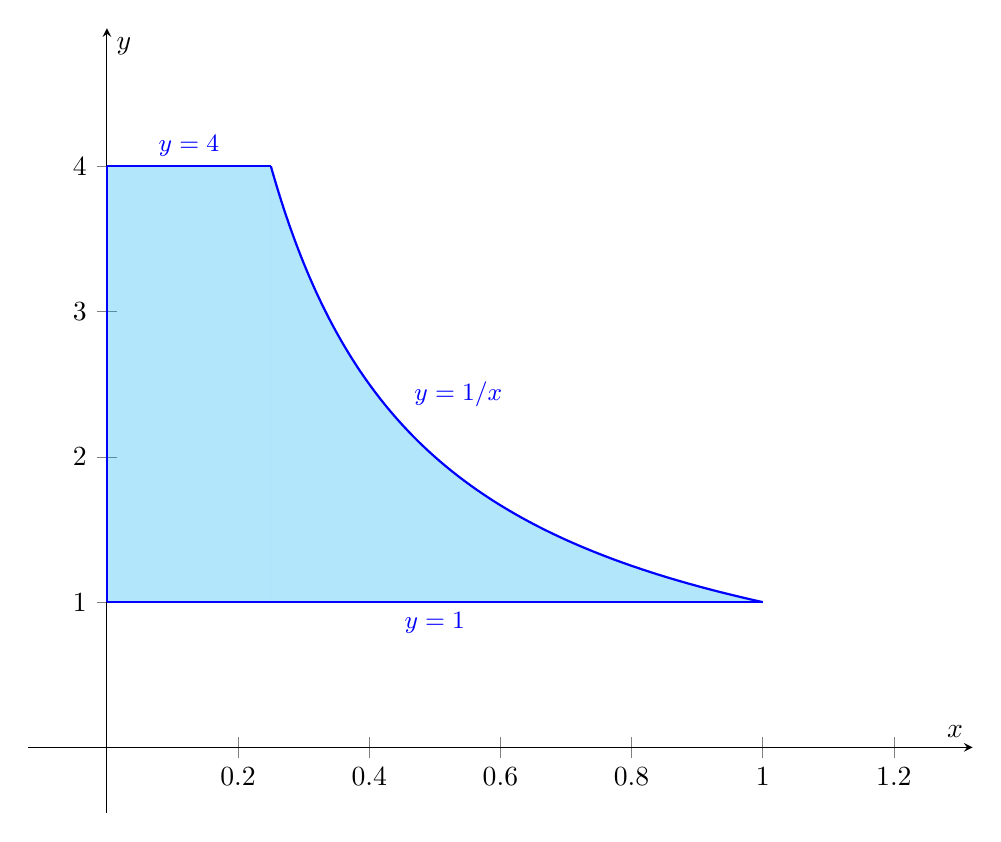
\begin{tikzpicture} [scale=1.75]
              \begin{axis}[
                  axis lines=middle,
                  xlabel=$x$,
                  ylabel=$y$,
                  xmin=0, xmax=1.2,
                  ymin=0, ymax=4.5,
                  enlargelimits=true,
                  title style={anchor=south, yshift=1ex}
                ]

                % Define the boundary curves
                % 1. The curve y = 1/x
                \addplot [name path=curve, domain=0.25:1, samples=1000, blue, thick] {1/x}
                node[right, xshift=10pt, pos=0.5, font=\small] {$y=1/x$};

                % 2. The bottom line y = 1
                \addplot [name path=bottom, domain=0:1, samples=20, blue, thick] {1}
                node[below, pos=0.5, font=\small] {$y=1$};

                % 3. The top line y = 4
                \addplot [name path=top, domain=0:0.25, samples=20, blue, thick] {4}
                node[above, pos=0.5, font=\small] {$y=4$};

                % 4. The left boundary x = 0 (y-axis)
                \draw [name path=left, samples=20, blue, thick] (axis cs:0,1) -- (axis cs:0,4);

                % Shade the region by breaking it into two parts at x=0.25
                % Part 1: The rectangle from x=0 to x=0.25
                \addplot [fill=cyan, opacity=0.3] fill between [
                  of=top and bottom,
                  soft clip={domain=0:0.25}
                ];

                % Part 2: The area under the curve from x=0.25 to x=1
                \addplot [fill=cyan, opacity=0.3] fill between [
                  of=curve and bottom,
                  soft clip={domain=0.25:1}
                ];
              \end{axis}
            \end{tikzpicture}
          \end{center}
        \end{answerbox}
        \vspace{0.5 in}
      \item[(b)] Evaluate the integral.
        \newline

        \begin{answerbox}
          To evaluate the integral
          \[
            \int_1^4 \int_0^{1/y} \frac{x}{y} \, dx \, dy,
          \]
          we first compute the inner integral with respect to \(x\):
          \[
            \int_0^{1/y} \frac{x}{y} \, dx = \frac{1}{y} \int_0^{1/y} x \, dx = \frac{1}{y} \left[ \frac{x^2}{2} \right]_0^{1/y} = \frac{1}{y} \cdot \frac{(1/y)^2}{2} = \frac{1}{2y^3}.
          \]
          Now we substitute this result into the outer integral:
          \[
            \int_1^4 \frac{1}{2y^3} \, dy = \frac{1}{2} \int_1^4 y^{-3} \, dy.
          \]
          We compute the integral:
          \[
            \int y^{-3} \, dy = \int y^{-3} \, dy = -\frac{1}{2y^2} + C.
          \]
          Evaluating this from 1 to 4 gives:
          \[
            \left[ -\frac{1}{2y^2} \right]_1^4 = -\frac{1}{2(4^2)} + \frac{1}{2(1^2)} = -\frac{1}{32} + \frac{1}{2} = \frac{16}{32} - \frac{1}{32} = \frac{15}{32}.
          \]
          Therefore, the value of the integral is:
          \[
            \frac{1}{2} \cdot \frac{15}{32} = \frac{15}{64}.
          \]
          Thus, the final answer is:
          \[
            \frac{15}{64}.
          \]
        \end{answerbox}
    \end{itemize}

    \vspace{0.5 in}
  \item[6.] Consider the iterated integral
    \begin{align*}
      \int_0^4\int_{\sqrt{x}}^2\sin(y^3) dydx.
    \end{align*}

    \smallskip
    \begin{itemize}
      \item[(a)] Sketch the region determined by the bounds of the integral.
        \newline

        \begin{answerbox}
          \begin{center}
            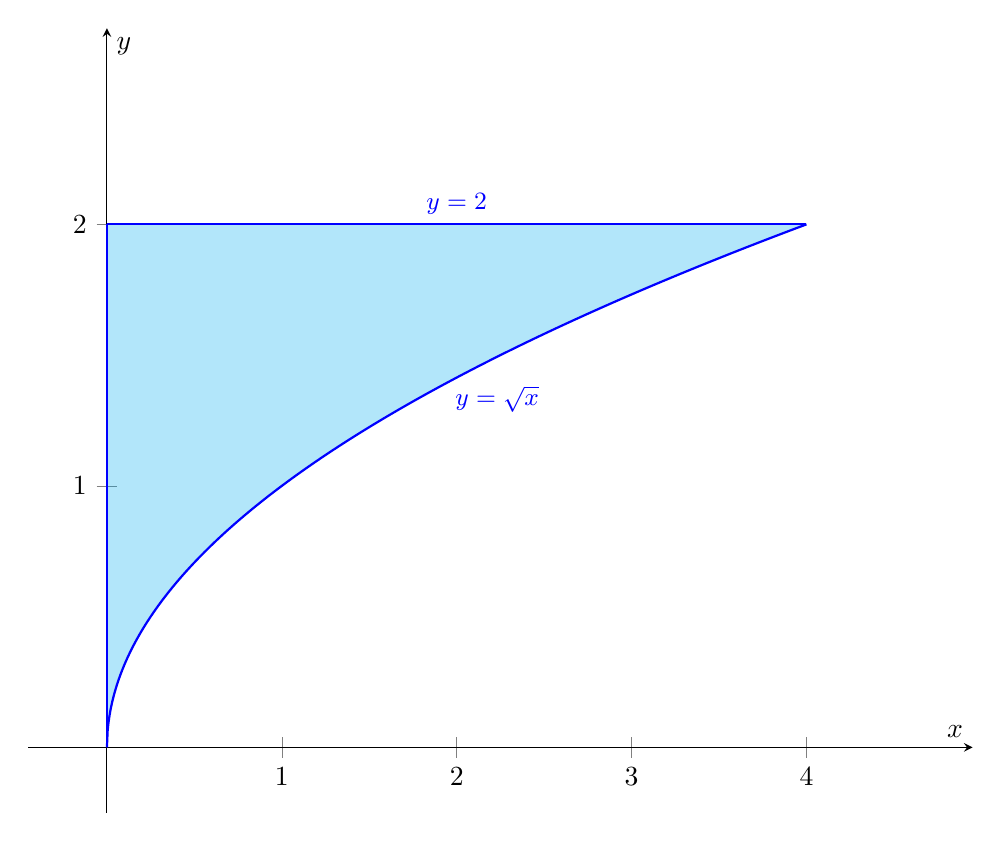
\begin{tikzpicture} [scale=1.75]
              \begin{axis}[
                  axis lines=middle,
                  xlabel=$x$,
                  ylabel=$y$,
                  xmin=0, xmax=4.5,
                  ymin=0, ymax=2.5,
                  enlargelimits=true,
                  % title={Region for Problem 6(a)},
                  title style={anchor=south, yshift=1ex}
                ]

                % Define the boundary curves
                % 1. The curve y = sqrt(x)
                \addplot [name path=curve, domain=0:4, samples=1000, blue, thick] {sqrt(x)}
                node[right, xshift=10pt, pos=0.5, font=\small] {$y=\sqrt{x}$};

                % 2. The top line y = 2
                \addplot [name path=top, domain=0:4, samples=20, blue, thick] {2}
                node[above, pos=0.5, font=\small] {$y=2$};

                % 3. The left boundary x = 0 (y-axis)
                \draw [name path=left, samples=20, blue, thick] (axis cs:0,0) -- (axis cs:0,2);

                % Shade the region between the curve and the line
                \addplot [fill=cyan, opacity=0.3] fill between [
                  of=top and curve,
                  soft clip={domain=0:4}
                ];
              \end{axis}
            \end{tikzpicture}
          \end{center}
        \end{answerbox}
        \vspace{0.5 in}
        \newpage
      \item[(b)] Evaluate the integral by reversing the order of integration.
        \newline

        \begin{answerbox}
          To reverse the order of integration for the integral
          \[
            \int_0^4 \int_{\sqrt{x}}^2 \sin(y^3) \, dy \, dx,
          \]
          we first identify the region of integration. The bounds indicate that \(x\) ranges from 0 to 4, and for each fixed \(x\), \(y\) ranges from \(\sqrt{x}\) to 2.

          Rewriting the bounds in terms of \(y\):
          - The lower bound for \(y\) is \(\sqrt{x}\), which implies \(x = y^2\).
          - The upper bound for \(y\) is 2, which implies \(x\) can go up to 4.

          Thus, for a fixed \(y\), \(x\) ranges from 0 to \(y^2\). The new bounds for \(y\) are from 0 to 2. Therefore, the reversed integral is:
          \[
            \int_0^2 \int_0^{y^2} \sin(y^3) \, dx \, dy.
          \]

          Now we evaluate the inner integral with respect to \(x\):
          \[
            \int_0^{y^2} \sin(y^3) \, dx = \sin(y^3) \cdot (y^2 - 0) = y^2 \sin(y^3).
          \]

          Substituting this into the outer integral gives:
          \[
            \int_0^2 y^2 \sin(y^3) \, dy.
          \]

          To evaluate this integral, we use the substitution \(u = y^3\), which gives \(du = 3y^2 dy\) or \(y^2 dy = \frac{du}{3}\). When \(y = 0\), \(u = 0\), and when \(y = 2\), \(u = 8\). Thus, the integral becomes:
          \[
            \int_0^8 \sin(u) \cdot \frac{1}{3} \, du = \frac{1}{3} \int_0^8 \sin(u) \, du.
          \]

          Evaluating this integral:
          \[
            \frac{1}{3} \left[ -\cos(u) \right]_0^8 = \frac{1}{3} \left( -\cos(8) + \cos(0) \right) = \frac{1}{3} \left(1 - \cos(8) \right).
          \]
          Therefore, the value of the integral is:
          \[
            \frac{1 - \cos(8)}{3}.
          \]
        \end{answerbox}
    \end{itemize}

\end{itemize}
\end{document}
